\subsection{Radiative Cooling and Heating}
\label{sec.num.cooling}

\enzo has multiple methods for computing the energy change from
radiative cooling and heating.  All of them assume the gas is totally
optically thin.  Below we describe the methods for computing the
cooling rates from metal-free and metal-enriched gas.  Sample cooling
curves for each of \enzo's primary cooling methods are shown in Figure
\ref{fig.cooling}.

\subsubsection{Primordial Cooling}

As discussed in \S\ref{sec.ov.chem}, the set of reactions that
characterize a metal-free gas is simple enough to be computed in
non-equilibrium during the simulation.  Similarly, the radiative
cooling of metal-free gas is solved by directly computing the cooling
and heating rates from the following individual processes for atomic
H and He: collisional excitation and ionization, recombination,
free-free emission, Compton scattering off of the cosmic microwave
background (CMB), and photo-heating from a UV metagalactic background.
If the H$_{2}$ chemistry network is enabled, the following H$_{2}$
cooling processes are also considered: ro-vibrational transitions 
\citep{1998A&A...335..403G}, heating and cooling from molecular
formation and destruction \citep{2009Sci...325..601T}, and 
collision-induced emission \citep{2004MNRAS.348.1019R}.  If Deuterium
chemistry is enabled, then rotational transitions of HD
\citep{1998A&A...335..403G} are treated as well.  The radiative
cooling calculation is coupled to the update of the chemistry network
such that they both occur within the same subcycling loop.  In
addition to the subcycle timestepping contraints mentioned in
\S\ref{sec.ov.chem}, the subcycle timestep is also not permitted to
exceed 10\% of the cooling time, $e/\dot{e}$.  A metagalactic
background affects the gas through both photo-heating and
photo-ionization.  These are treated by including redshift-dependent 
photo-ionization and photo-heating rate terms in the chemistry and
cooling equations for HI, HeI, and HeII.  More detail on the specific
UV backgrounds present in \enzo is given below.

\subsubsection{Metal Cooling}



\begin{figure} \label{fig.cooling}
  \begin{center}
    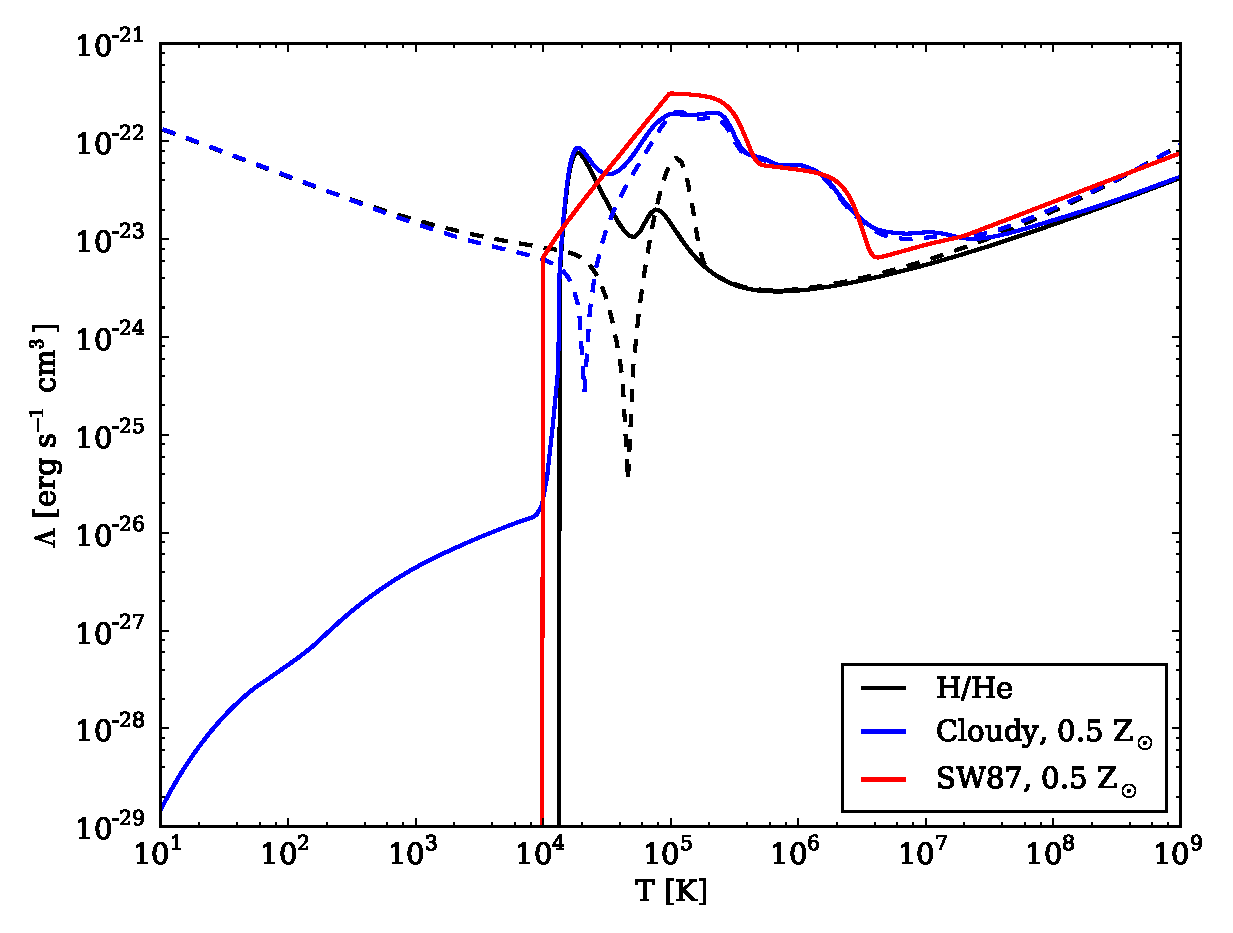
\includegraphics[width=1.0\textwidth]{figures/cooling_rate.eps}
    \caption{Radiative cooling rates from the various cooling methods
      available in \enzo.  The black curves show cooling rates from a gas
      with primordial composition using the non-equilibrium chemistry
      network.  The blue curves are for a gas with metallicity of 0.5
      $Z_{\odot}$ computed with the Cloudy cooling method.  The solid
      black and blue lines assume collisional processes only while the
      dashed lines include photo-ionization and photo-heating from a UV
      metagalactic background at $z = 0$ with a gas number density of
      10$^{-4}$ cm$^{-3}$.  The low temperature rates shown by the
      dashed lines indicate a net heating.  The red curve is the
      tabulated cooling function of \citet{SW87} which assumes a fully
      ionized gas with metallicity of 0.5 $Z_{\odot}$.}
  \end{center}
\end{figure}
